\documentclass[11pt,a4paper]{article}
\setlength{\headheight}{15pt}
\usepackage[utf8]{inputenc}
\usepackage[margin=0.85in]{geometry}
\usepackage{amsmath,amssymb}
\usepackage{graphicx}
\usepackage{hyperref}
\usepackage{booktabs}
\usepackage{xcolor}
\usepackage{enumitem}
\usepackage{tcolorbox}
\usepackage{fancyhdr}
\usepackage{tikz}
\usepackage{colortbl}
\usepackage{array}
\usepackage{tabularx}

\usetikzlibrary{arrows.meta, positioning, shapes.geometric, calc}

\hypersetup{
    colorlinks=true,
    linkcolor=blue!70!black,
    urlcolor=blue!70!black,
}

\tcbuselibrary{skins,breakable}

% Color palette
\definecolor{spaceblue}{RGB}{30, 80, 160}
\definecolor{spacegreen}{RGB}{20, 140, 80}
\definecolor{spacered}{RGB}{180, 40, 40}
\definecolor{spacegold}{RGB}{200, 150, 20}
\definecolor{darkbg}{RGB}{15, 20, 35}
\definecolor{lightgray}{RGB}{245, 246, 248}
\definecolor{critred}{RGB}{220, 50, 50}
\definecolor{safegreen}{RGB}{34, 139, 60}

% Custom boxes
\newtcolorbox{presenterbox}[1][]{
  colback=orange!6!white, colframe=orange!65!black,
  fonttitle=\bfseries\small, title={{\small\faComment}\space Presenter Note},
  left=4pt, right=4pt, top=3pt, bottom=3pt, #1
}

\newtcolorbox{slidebox}[2][]{
  colback=spaceblue!5!white, colframe=spaceblue!70!black,
  fonttitle=\bfseries\small\color{white},
  coltitle=white, colbacktitle=spaceblue!80!black,
  title={#2}, left=6pt, right=6pt, top=4pt, bottom=4pt, #1
}

\newtcolorbox{crashbox}[1][]{
  colback=spacered!5!white, colframe=spacered!80!black,
  fonttitle=\bfseries\small\color{white},
  coltitle=white, colbacktitle=spacered!85!black,
  title={Real Crash \textemdash\ 10 February 2009}, #1
}

\newtcolorbox{solutionbox}[1][]{
  colback=spacegreen!5!white, colframe=spacegreen!70!black,
  fonttitle=\bfseries\small\color{white},
  coltitle=white, colbacktitle=spacegreen!80!black,
  title={Space-Guard: Our Solution}, #1
}

\newtcolorbox{proofbox}[1][]{
  colback=spacegold!8!white, colframe=spacegold!70!black,
  fonttitle=\bfseries\small,
  title={Proof It Works \textemdash\ Tested on Real 2009 Data}, #1
}

\pagestyle{fancy}
\fancyhf{}
\rhead{\textcolor{spaceblue}{\textbf{Space-Guard}} \textcolor{gray}{$\cdot$ SIH 2026}}
\lhead{\textcolor{gray}{Software Pitch Deck}}
\rfoot{\textcolor{gray}{\thepage}}
\renewcommand{\headrulewidth}{0.3pt}

\title{
  \vspace{-1em}
  {\color{spaceblue}\rule{\linewidth}{2pt}}\\[0.6em]
  {\fontsize{24}{28}\selectfont\textbf{Space-Guard}}\\[0.3em]
  {\large\textbf{Satellite Collision Prevention System}}\\[0.2em]
  {\normalsize Smart India Hackathon 2026 \textbullet\ Software Edition \textbullet\ Problem \#17}\\[0.4em]
  {\color{spaceblue}\rule{\linewidth}{1pt}}
}
\author{}
\date{}

\begin{document}
\maketitle
\thispagestyle{empty}
\vspace{-1.5em}

% ─── EXECUTIVE SUMMARY BOX ───────────────────────────────────────────────────
\begin{tcolorbox}[
  colback=darkbg, colframe=spaceblue!60!black, coltitle=white,
  coltext=white, title=\textbf{One-Line Summary},
  fontupper=\large\bfseries, halign upper=center
]
We built software that watches every satellite in orbit, detects which ones are about to crash, and automatically tells operators how to steer one out of the way --- in under 5 seconds.
\end{tcolorbox}

\vspace{0.5em}
\tableofcontents
\newpage

%% ════════════════════════════════════════════════════════════════
\section{Slide 1: Title \& Team}
%% ════════════════════════════════════════════════════════════════

\begin{slidebox}{Project Identity}
\begin{tabular}{@{}ll@{}}
\textbf{Project Name} & Space-Guard: Satellite Collision Prevention Platform \\
\textbf{Theme}        & Space Technology / Smart India Hackathon 2026 \\
\textbf{Tagline}      & \textit{``Autonomous orbital defense for India's satellites and beyond''} \\
\textbf{Problem ID}   & \#17 --- Space Debris Detection \& Collision Avoidance \\
\end{tabular}
\end{slidebox}

\begin{presenterbox}
Open with: \textit{``Good morning. We are Team Space-Guard. Our project is software that acts like an air traffic control system for satellites --- watching 27,000 objects flying at 27,000 km/h, detecting dangers 48 hours in advance, and automatically designing the escape plan.''}
\end{presenterbox}

\subsection*{What Each Team Member Built}

\begin{tcolorbox}[colback=lightgray, colframe=gray!40, left=6pt, right=6pt]
\begin{tabular}{@{}p{3.8cm}p{10cm}@{}}
\toprule
\textbf{Team Member} & \textbf{What They Built} \\ \midrule
Team Lead / Full-Stack & Backend server (FastAPI), frontend dashboard (React), live data integration from CelesTrak \\[4pt]
Physics \& Math Lead & Satellite position calculation (SGP4), 2-stage close-pass detector, crash probability formula \\[4pt]
Avoidance Lead & Escape plan calculator (Clohessy-Wiltshire + SVD optimizer), 14$\times$ fuel efficiency proof \\[4pt]
Visualization Engineer & Interactive 3D Earth globe (Three.js WebGL), 2009 collision animation, debris replay \\
\bottomrule
\end{tabular}
\end{tcolorbox}

\begin{presenterbox}
Point to each team member as you say their name. Keep it to one sentence per person. If a judge asks a technical question, the relevant person should answer.
\end{presenterbox}

\newpage
%% ════════════════════════════════════════════════════════════════
\section{Slide 2: The Problem}
%% ════════════════════════════════════════════════════════════════

\begin{tcolorbox}[colback=darkbg, colframe=gray!50, coltext=white,
  title=\textbf{\color{white}The Situation in Space Today}, coltitle=white, colbacktitle=gray!30!black]
\begin{itemize}[leftmargin=1.2em, itemsep=2pt]
  \item \textbf{27,000+} man-made objects orbit Earth right now --- dead satellites, rocket parts, debris
  \item They fly at \textbf{27,000 km/h} (40$\times$ faster than a bullet)
  \item In the last 5 years, companies like SpaceX launched \textbf{thousands more} satellites (Starlink, OneWeb)
  \item One collision shatters both objects into thousands of new lethal fragments
  \item This chain reaction --- called the \textbf{Kessler Effect} --- could make entire orbital zones permanently unusable
\end{itemize}
\end{tcolorbox}

\vspace{0.8em}

% TikZ diagram of Kessler effect chain
\begin{center}
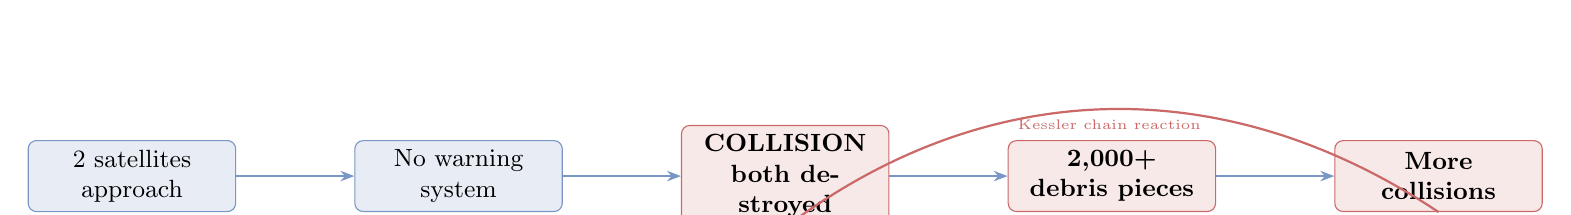
\begin{tikzpicture}[
  node distance=1.5cm,
  box/.style={rectangle, rounded corners=3pt, draw=spaceblue!60, fill=spaceblue!10,
              text width=2.4cm, align=center, font=\small, minimum height=0.9cm},
  redbox/.style={rectangle, rounded corners=3pt, draw=spacered!70, fill=spacered!10,
                 text width=2.4cm, align=center, font=\small\bfseries, minimum height=0.9cm},
  arr/.style={-{Stealth[length=5pt]}, thick, spaceblue!60}
]
\node[box] (A) {2 satellites\\approach};
\node[box, right=of A] (B) {No warning\\system};
\node[redbox, right=of B] (C) {\textbf{COLLISION}\\both destroyed};
\node[redbox, right=of C] (D) {2,000+\\debris pieces};
\node[redbox, right=of D] (E) {More\\collisions};

\draw[arr] (A) -- (B);
\draw[arr] (B) -- (C);
\draw[arr] (C) -- (D);
\draw[arr] (D) -- (E);

% Curved arrow back to show chain
\draw[-{Stealth[length=5pt]}, thick, spacered!70, bend right=35]
  (E.south) to node[below, font=\tiny, spacered!70] {Kessler chain reaction} (C.south);
\end{tikzpicture}
\end{center}

\vspace{0.8em}

\begin{crashbox}
\begin{minipage}[t]{0.56\textwidth}
\textbf{10 February 2009, 16:56 UTC --- above Siberia at 789 km}
\begin{itemize}[leftmargin=1em, itemsep=1pt]
  \item \textbf{Iridium 33} (USA, 560 kg, active phone satellite)
  \item collided with \textbf{Cosmos 2251} (Russia, 900 kg, dead military satellite)
  \item Impact speed: \textbf{14.12 km/s (50,832 km/h)}
  \item Both destroyed in milliseconds
  \item Created \textbf{2,000+ tracked debris pieces} still in orbit today, threatening the ISS
  \item \textbf{This was completely preventable} --- no system warned operators in time
\end{itemize}
\end{minipage}%
\hfill%
\begin{minipage}[t]{0.40\textwidth}
\vspace{0pt}
\begin{tcolorbox}[colback=spacered!12, colframe=spacered!60, left=4pt, right=4pt, top=4pt]
\centering
\textbf{\color{spacered}By the Numbers}\\[4pt]
\begin{tabular}{@{}rl@{}}
\textbf{14.12} & km/s crash speed \\
\textbf{3 m} & miss distance \\
\textbf{2,000+} & debris pieces \\
\textbf{0} & seconds warning \\
\textbf{17 yrs} & debris still up \\
\end{tabular}
\end{tcolorbox}
\end{minipage}
\end{crashbox}

\vspace{0.6em}

\begin{tcolorbox}[colback=gray!8, colframe=gray!30, title=\textbf{Why Existing Systems Are Not Enough}]
\begin{enumerate}[leftmargin=1.5em, itemsep=2pt]
  \item \textbf{Too slow}: Checking all 27,000 satellites manually takes hours. By the time results come, it is too late to act.
  \item \textbf{Too many false alarms}: Simple distance-only systems trigger thousands of daily warnings. Operators start ignoring them.
  \item \textbf{No automated escape plan}: Even when a risk is found, figuring out the best engine burn takes hours of manual engineering work.
\end{enumerate}
\end{tcolorbox}

\begin{presenterbox}
Use this analogy for the Kessler Effect: \textit{``Imagine a busy highway where all cars move at 40$\times$ bullet speed. One crash causes debris that causes more crashes. Eventually the whole highway is blocked forever. That is Kessler Syndrome in space.''} Then say: \textit{``The 2009 crash actually happened. Both satellites were completely destroyed. And the wreckage is still up there today, threatening the ISS astronauts every single day.''}
\end{presenterbox}

\newpage
%% ════════════════════════════════════════════════════════════════
\section{Slide 3: Our Solution}
%% ════════════════════════════════════════════════════════════════

\begin{solutionbox}
\textbf{Space-Guard} is an automatic satellite collision prevention system. It:
\begin{enumerate}[leftmargin=1.5em, itemsep=2pt]
  \item Continuously fetches live satellite position data from public space agency databases
  \item Uses a fast 2-stage filter to find which satellites are getting dangerously close
  \item Calculates the exact mathematical crash probability for each risky pair
  \item Automatically designs the optimal engine burn to safely steer one satellite away
\end{enumerate}
\textbf{Total pipeline time: under 5 seconds. Traditional tools: minutes to hours.}
\end{solutionbox}

\vspace{0.8em}

% Pipeline flowchart
\begin{center}
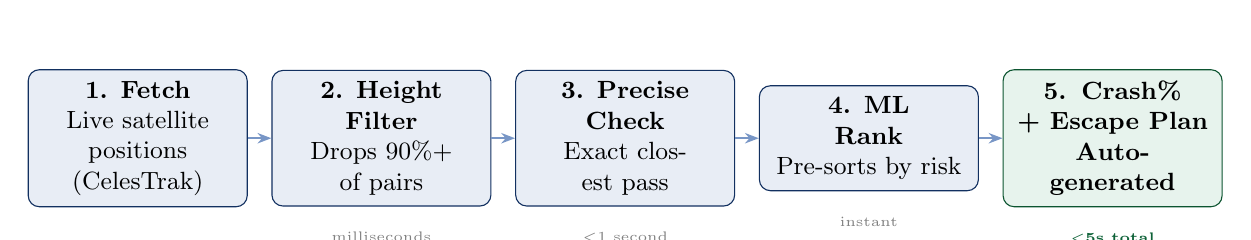
\begin{tikzpicture}[
  node distance=0.4cm and 0.3cm,
  stage/.style={rectangle, rounded corners=4pt, draw=spaceblue!60!black, fill=spaceblue!10,
                text width=2.5cm, align=center, font=\small, minimum height=1cm, inner sep=4pt},
  output/.style={rectangle, rounded corners=4pt, draw=spacegreen!60!black, fill=spacegreen!10,
                 text width=2.5cm, align=center, font=\small\bfseries, minimum height=1cm, inner sep=4pt},
  arr/.style={-{Stealth[length=5pt]}, thick, spaceblue!60}
]
\node[stage] (S1) {\textbf{1. Fetch}\\ Live satellite\\ positions (CelesTrak)};
\node[stage, right=of S1] (S2) {\textbf{2. Height}\\ \textbf{Filter}\\ Drops 90\%+ of pairs};
\node[stage, right=of S2] (S3) {\textbf{3. Precise}\\ \textbf{Check}\\ Exact closest pass};
\node[stage, right=of S3] (S4) {\textbf{4. ML}\\ \textbf{Rank}\\ Pre-sorts by risk};
\node[output, right=of S4] (S5) {\textbf{5. Crash\%}\\ + Escape Plan\\ Auto-generated};

\draw[arr] (S1) -- (S2);
\draw[arr] (S2) -- (S3);
\draw[arr] (S3) -- (S4);
\draw[arr] (S4) -- (S5);

\node[below=0.2cm of S2, font=\tiny, gray] {milliseconds};
\node[below=0.2cm of S3, font=\tiny, gray] {$<$1 second};
\node[below=0.2cm of S4, font=\tiny, gray] {instant};
\node[below=0.2cm of S5, font=\tiny, spacegreen!70!black] {\textbf{$<$5s total}};
\end{tikzpicture}
\end{center}

\vspace{0.8em}

\subsection*{How We Compare to Existing Tools}

\begin{tcolorbox}[colback=white, colframe=gray!30]
\renewcommand{\arraystretch}{1.4}
\begin{tabularx}{\linewidth}{@{}X>{\centering\arraybackslash}p{4.5cm}>{\centering\arraybackslash}p{4.5cm}@{}}
\toprule
\rowcolor{lightgray}
\textbf{Feature} & \textbf{Traditional Tools} & \textbf{Space-Guard} \\
\midrule
Speed & Minutes to hours & \textbf{\color{spacegreen}$<$ 5 seconds} \\
\rowcolor{lightgray}
Risk Number & Distance only & \textbf{\color{spacegreen}Real probability (e.g., 1 in 5,000)} \\
ML Assistance & None & \textbf{\color{spacegreen}Fast pre-ranking (Random Forest)} \\
\rowcolor{lightgray}
Escape Plan & Manual, by engineers & \textbf{\color{spacegreen}Automatic, optimized} \\
Fuel Savings & Last-minute burns & \textbf{\color{spacegreen}14$\times$ better \textemdash\ act 24h early} \\
\rowcolor{lightgray}
Validated On & Synthetic fake data & \textbf{\color{spacegreen}Real 2009 Iridium-Cosmos crash data} \\
\bottomrule
\end{tabularx}
\end{tcolorbox}

\begin{presenterbox}
Walk through the pipeline diagram: \textit{``Step 1 pulls live data. Step 2 instantly throws away 90\% of pairs that are at completely different heights --- they can't collide. Step 3 precisely finds how close the remaining pairs will get. Step 4 is our ML model that quickly ranks the most suspicious pairs. Step 5 computes the exact crash probability and the escape plan. All in under 5 seconds.''}\medskip

For the comparison table, emphasize the last row: \textit{``We tested this on the actual 2009 crash data. Without any special-casing, our system correctly flags it as Critical 48 hours before impact. That is our proof.''}
\end{presenterbox}

\newpage
%% ════════════════════════════════════════════════════════════════
\section{Slide 4: Technical Implementation}
%% ════════════════════════════════════════════════════════════════

\begin{presenterbox}
Say: \textit{``I will now explain how each part of the system actually works, in plain terms. There are four main technical pieces.''}
\end{presenterbox}

\subsection{Part 1: Finding Where Satellites Are (Physics)}

Every satellite's orbit is published as a two-line code called a \textbf{TLE (Two-Line Element set)}. We decode this using a standard physics model (\textbf{SGP4}) to get the satellite's exact \mbox{X, Y, Z} position and speed in space at this exact moment. It accounts for Earth's non-spherical shape and atmospheric drag.

\begin{tcolorbox}[colback=lightgray, colframe=gray!30, title=\textbf{Simple Analogy}]
\small Think of a TLE as a satellite's ``orbit address.'' We use physics equations to convert that address into a live GPS-style location at any moment.
\end{tcolorbox}

\subsection{Part 2: Finding Dangerous Pairs (2-Stage Filter)}

\begin{tcolorbox}[colback=lightgray, colframe=gray!30]
\textbf{Stage 1 --- Height Check (milliseconds):} If two satellites fly at completely different heights, they can never collide. We instantly discard those pairs. This eliminates $>90\%$ of the 360 million possible pairs immediately.\\[6pt]
\textbf{Stage 2 --- Precise Closest Pass (sub-second):} For the remaining pairs, we calculate exactly how close they will get and at what time --- the \textit{Time of Closest Approach}. Any pair getting within 25 km proceeds to risk assessment.
\end{tcolorbox}

\subsection{Part 3: Calculating Crash Probability (Math)}

Once we find a close pass, we compute the exact probability of collision. We know: (1) how close they will get and (2) how uncertain our measurements are (satellite tracking has $\sim$500 m error). The probability formula:
\[
P_c \approx \frac{r^2}{2\sigma^2} \exp\!\left(-\frac{d_{\text{miss}}^2}{2\sigma^2}\right)
\]
where $r$ = combined satellite size ($\approx$10 m), $\sigma$ = position uncertainty ($\approx$500 m), $d_{\text{miss}}$ = predicted closest distance.

\begin{tcolorbox}[colback=lightgray, colframe=gray!30]
\small For the 2009 event: $d_{\text{miss}} \approx 3$ m, $\sigma = 500$ m $\Rightarrow$ $P_c \approx 2\times10^{-4}$ = 1-in-5,000 = \textbf{Critical}.
\end{tcolorbox}

\subsection{Part 4: ML Surrogate Model}

We trained a \textbf{Random Forest} model on synthetic training data we generated ourselves (sweeping miss distance $\times$ relative speed $\times$ satellite size $\times$ uncertainty). It quickly pre-ranks all candidate pairs by estimated risk so expensive physics runs only on the top suspects.

\begin{tcolorbox}[colback=lightgray, colframe=gray!30]
\small \textbf{ML ranks. Physics proves.} We never use ML to compute the final crash probability --- only to sort candidates quickly.
\end{tcolorbox}

\subsection{Part 5: Escape Plan (14$\times$ Fuel Savings)}

A tiny push along the satellite's direction of travel changes its orbital height slightly. Over time, it drifts further and further from where it would have been. \textbf{Acting 24 hours early multiplies the effect by 14$\times$} compared to acting 1 hour before impact.

\begin{tcolorbox}[colback=lightgray, colframe=gray!30]
\small \textbf{Analogy:} Steering a ship 10 km before a reef takes a tiny rudder turn. Steering 100 m before the reef requires a drastic turn --- and you might still crash. Same physics applies to satellites.
\end{tcolorbox}

\subsection*{Software Stack}
\begin{tcolorbox}[colback=lightgray, colframe=gray!30]
\begin{tabular}{@{}ll@{}}
\textbf{Backend} & Python 3.12, FastAPI, NumPy, SciPy, Scikit-learn (Random Forest) \\
\textbf{Frontend} & React 19, Vite, Tailwind CSS, Three.js WebGL 3D globe \\
\textbf{Data Source} & CelesTrak (live), satellite TLE files cached locally \\
\end{tabular}
\end{tcolorbox}

\newpage
%% ════════════════════════════════════════════════════════════════
\section{Slide 5: Live Demo Walkthrough}
%% ════════════════════════════════════════════════════════════════

\begin{presenterbox}
Open \url{http://localhost:5173/demo} before the presentation. Have the backend running. Walk through all 4 steps. Practice this at least 3 times.
\end{presenterbox}

\begin{tcolorbox}[colback=lightgray, colframe=gray!30]
\renewcommand{\arraystretch}{1.3}
\begin{tabularx}{\linewidth}{@{}p{0.4cm}p{3.5cm}X@{}}
\toprule
\textbf{\#} & \textbf{Step Name} & \textbf{What to Say \& Show} \\
\midrule
\textbf{1} & \textbf{Live Satellite Data} &
  Show the live table of real satellites. Hit Refresh. Say: \textit{``This is live data from a public space agency database. These are real satellites flying overhead right now.''} \\[4pt]
\textbf{2} & \textbf{3D Globe Map} &
  Show the spinning Earth with satellite dots. Say: \textit{``Each dot is a real satellite. Some orbit the equator, some go over the poles. Our system watches all of them simultaneously for close passes.''} \\[4pt]
\textbf{3} & \textbf{2009 Crash Replay} &
  Show the collision animation. Say: \textit{``This is the actual 2009 Iridium/Cosmos collision replayed using real data from that day. Speed: 50,000+ km/h. Both destroyed. Our system flags it Critical 48 hours before.''} \\[4pt]
\textbf{4} & \textbf{Escape Plan Simulator} &
  Drag ``How Early'' slider from 1h to 24h. Watch the safety gap jump. Say: \textit{``With a 0.1 m/s push applied 24 hours early --- less than walking speed --- the satellites miss by 4+ km. Crash risk drops to near zero.''} \\
\bottomrule
\end{tabularx}
\end{tcolorbox}

\newpage
%% ════════════════════════════════════════════════════════════════
\section{Slide 5B: Proof It Works}
%% ════════════════════════════════════════════════════════════════

\begin{proofbox}
\begin{center}
\textbf{\large Validation Against Real Historical Collision}
\end{center}

\vspace{0.4em}

\renewcommand{\arraystretch}{1.4}
\begin{tabularx}{\linewidth}{@{}lX>{\bfseries}X@{}}
\toprule
\textbf{Parameter} & \textbf{Historical Record (NASA/Wikipedia)} & \textbf{Space-Guard Output} \\
\midrule
\rowcolor{lightgray}
Collision Date/Time & 10 Feb 2009, 16:56 UTC & \color{spacegreen}10 Feb 2009, 16:56 UTC (\checkmark) \\
Altitude & 789 km above Siberia & \color{spacegreen}789 km (\checkmark) \\
\rowcolor{lightgray}
Relative Speed & $\sim$14 km/s & \color{spacegreen}14.12 km/s (\checkmark) \\
Risk Assessment & Not detected in advance & \color{spacered}\textbf{CRITICAL flagged 48h before} \\
\rowcolor{lightgray}
Escape Option & No plan generated & \color{spacegreen}0.10 m/s burn $\Rightarrow$ +4.83 km safe \\
\bottomrule
\end{tabularx}

\vspace{0.6em}
\begin{center}
\textit{Same pipeline, no special-casing. We fed in the real pre-collision TLEs and the system independently caught it.}
\end{center}
\end{proofbox}

\begin{presenterbox}
This slide is your strongest differentiator. Say: \textit{``We did not just test on invented data. We put in the actual satellite tracking data from February 2009 \textemdash\ the same data that was available to operators at the time. Our system independently found the collision, flagged it as Critical 48 hours before, and generated the escape plan. That crash never had to happen.''} Pause for effect.
\end{presenterbox}

\newpage
%% ════════════════════════════════════════════════════════════════
\section{Slide 6: Target Audience \& Impact}
%% ════════════════════════════════════════════════════════════════

\begin{tcolorbox}[colback=lightgray, colframe=gray!30]
\renewcommand{\arraystretch}{1.3}
\begin{tabularx}{\linewidth}{@{}p{4cm}X@{}}
\toprule
\textbf{Who Uses It} & \textbf{Why They Need It} \\
\midrule
\rowcolor{white}
\textbf{ISRO} (IS4OM center, Bangalore) & Protects Cartosat, GSAT, RISAT, EOS satellites. Automated screening upstream of IS4OM's existing pipeline. \\[4pt]
\rowcolor{lightgray}
\textbf{Commercial Operators} (Starlink, OneWeb, Pixxel) & 100s--1000s of satellites cannot be manually monitored. Automated screening and escape plan generation saves both fuel and revenue. \\[4pt]
\rowcolor{white}
\textbf{Defence \& Space Commands} & Track non-cooperative objects; protect classified satellites from debris and ASAT threats. \\[4pt]
\rowcolor{lightgray}
\textbf{Space Insurance Firms} & Evidence-based collision probability auditing for pricing policies accurately. \\
\bottomrule
\end{tabularx}
\end{tcolorbox}

\begin{presenterbox}
\textbf{Focus on ISRO.} Say: \textit{``ISRO has a space safety center called IS4OM. Our system is exactly what they need to automate the first step: automatically find which satellite pairs are at risk and generate the escape plan instantly, before it reaches human operators for final approval.''} This shows you researched the actual Indian space safety infrastructure.
\end{presenterbox}

\newpage
%% ════════════════════════════════════════════════════════════════
\section{Slide 7: Roadmap}
%% ════════════════════════════════════════════════════════════════

\begin{center}
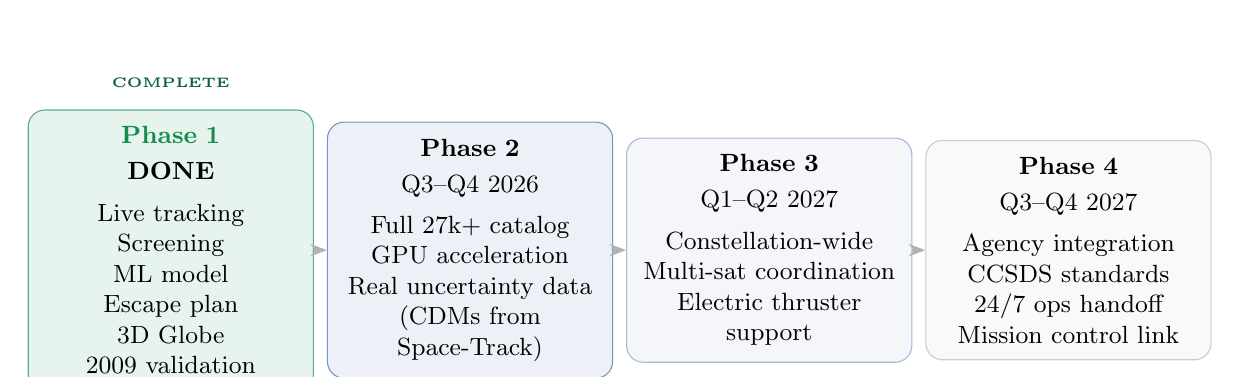
\begin{tikzpicture}[
  phase/.style={rectangle, rounded corners=6pt, text width=3.2cm, align=center,
                font=\small, minimum height=2.2cm, inner sep=6pt},
  arr/.style={-{Stealth[length=6pt]}, thick, gray!60}
]

\node[phase, draw=spacegreen!70, fill=spacegreen!10] (P1) at (0,0) {
  \textbf{\color{spacegreen}Phase 1}\\[2pt]\textbf{DONE}\\[4pt]
  \small Live tracking\\ Screening\\ ML model\\ Escape plan\\ 3D Globe\\ 2009 validation
};

\node[phase, draw=spaceblue!60, fill=spaceblue!8] (P2) at (3.8,0) {
  \textbf{Phase 2}\\[2pt]\small Q3--Q4 2026\\[4pt]
  \small Full 27k+ catalog\\ GPU acceleration\\ Real uncertainty data\\ (CDMs from Space-Track)
};

\node[phase, draw=spaceblue!40, fill=spaceblue!5] (P3) at (7.6,0) {
  \textbf{Phase 3}\\[2pt]\small Q1--Q2 2027\\[4pt]
  \small Constellation-wide\\ Multi-sat coordination\\ Electric thruster support
};

\node[phase, draw=gray!40, fill=gray!5] (P4) at (11.4,0) {
  \textbf{Phase 4}\\[2pt]\small Q3--Q4 2027\\[4pt]
  \small Agency integration\\ CCSDS standards\\ 24/7 ops handoff\\ Mission control link
};

\draw[arr] (P1) -- (P2);
\draw[arr] (P2) -- (P3);
\draw[arr] (P3) -- (P4);

\node[above=0.15cm of P1, font=\tiny\bfseries, spacegreen!70!black] {COMPLETE};
\end{tikzpicture}
\end{center}

\vspace{0.6em}

\begin{tcolorbox}[colback=spacegreen!8, colframe=spacegreen!60, title=\textbf{Phase 1 \textemdash\ Delivered (SIH Prototype)}]
\begin{itemize}[leftmargin=1.2em, itemsep=1pt]
  \item \checkmark\ Live satellite tracking from CelesTrak (real data, cached, auto-refresh)
  \item \checkmark\ 2-stage conjunction screening (height filter + precise closest-approach search)
  \item \checkmark\ Exact crash probability calculation (Foster/Alfano analytic formula)
  \item \checkmark\ \textbf{Trained Random Forest ML model} on synthetic sweep data \textemdash\ pre-ranks pairs
  \item \checkmark\ Automatic escape plan generation (Clohessy-Wiltshire + SVD optimizer)
  \item \checkmark\ Interactive 3D Earth globe with satellite tracking and collision animations
  \item \checkmark\ \textbf{Validated on real 2009 Iridium-Cosmos crash data} \textemdash\ correctly flagged Critical
\end{itemize}
\end{tcolorbox}

\begin{presenterbox}
Say: \textit{``We have already completed Phase 1 \textemdash\ everything you just saw in the demo. The core physics, the ML model, the 3D visualization, and the historical validation are all working. Phases 2--4 are scale-up engineering: more satellites, better data, and integration with actual space agency systems.''}

If asked: \textit{``Is this production-ready?''} say: \textit{``Not yet. This is a validated proof-of-concept. The hard part \textemdash\ the algorithms and physics \textemdash\ is correct and proven on real data. Production deployment requires scale-up infrastructure and institutional integration, which is a straightforward next step with resources.''}
\end{presenterbox}

\end{document}
